\subsection{Captura y validación de movimientos}

\subsubsection{Introducción}
En la aplicación de Practicante, se realiza el mismo proceso de captura que en la aplicación de Entrenador (ver sección \ref{sec:Captura} \nameref{sec:Captura}). El archivo con la información capturada se compara con el archivo capturado por el Entrenador obtenido de la base de datos. Se realizan diferentes capturas de acuerdo al número de repeticiones que indique la rutina. Cada una de esas capturas se compara con la del Entrenador y el resultado promedio de cada movimiento se guarda en la base de datos. Al término de la realización de una rutina, se calcula y muestra un desempeño al Practicante en términos de porcentaje, el cual indica su rendimiento general.\\

\subsubsection{Animaciones}
Existen diferentes aplicaciones para realizar captura de movimientos, sin embargo cada una ellas ofrece características particulares que se adaptan a diferentes necesidades. Se opta por hacer uso de estas herramientas para la creación de animaciones de manera que la curva de aprendizaje de la creación de animaciones no pueda representar un riesgo en la realización del Trabajo Terminal.\\

\textbf{Brekel.} Brekel Pro Body es una aplicación de Windows que les permite a los animadores de 3D hacer Motion Capture de hasta 2 personas en una habitación u oficina utilizando un sensor de Microsoft Kinect \cite{Brekel}. \\

\textbf{Características principales}

\begin{itemize} \itemsep1pt \parskip0pt \parsep0pt
	\item Utiliza el SDK de Microsoft Kinect. 
	\item Trabaja en tiempo real, no se requiere seguimiento en línea.
	\item Tiene soporte para rotación de manos, pies y cabeza.
	\item Escribe directamente los archivos en el disco duro en los formatos FBX, BVH y TXT.
	\item El reconocimiento de personas es muy veloz.
	\item Soporta el seguimiento de 2 personas.
	\item Opcionalmente puede reproducirse y grabar directamente en Autodesk MotionBuilder utilizando plugins para 2009-2016 y las versiones de 32 y 64 bits.
	\item Opcionalmente se puede reproducir directamente en el motor de gráfico Unity3D utilizando un script en c\# incluido. (Se necesitaran ajustes para tu propio rig).
	\item Viene con en script de ejemplo de  Maya MEL para importar en formato de texto.
	\item La versión de prueba se puede abrir hasta 100 veces antes de expirar.
	\item Si se utiliza por 5 días de seguidos también expira la licencia de prueba.
\end{itemize}
	
\textbf{Requisitos mínimos de hardware}

\begin{itemize} \itemsep1pt \parskip0pt \parsep0pt
	\item ``Kinect para Windows", o sensor ``Kinect para XBox"
	\item Microsoft Windows 7/8
	\item Procesador de 32 bits (x86) o 64 bits (x64)
	\item Procesador Intel Core i5 o superior(o equivalente)
	\item 4 GB RAM
	\item Tarjeta gráfica que soporte OpenGL
\end{itemize}

\textbf{iPi Recorder.} iPi Recorder es un software gratuito provisto por iPi Soft LLC para la captura, reproducción y procesamiento de grabaciones de video de múltiples cámaras y sensores de profundidad. Los grabaciones capturadas se pueden utilizar para seguimiento de movimientos en el software iPi Mocap Studio. \cite{iPi}\\

\textbf{Características principales}

\begin{itemize} \itemsep1pt \parskip0pt \parsep0pt
	\item SO Windows 8.1\/8\/7 (32 y 64 bits). 
	\item Camaras soportadas: 
	\begin{itemize} \itemsep1pt \parskip0pt \parsep0pt
		\item Sony PlayStation3 Eye.
		\item Kinect 2 para Windows\/Xbox One.
		\item Kinect para Windows\/Xbox 360.
		\item ASUS Xtion\/PrimeSense Carmine 1.08.
	\end{itemize}
	\item Controles de movimiento soportados:
	\begin{itemize} \itemsep1pt \parskip0pt \parsep0pt
		\item PlayStation Move.
		\item Wii Remote con MotionPlus.
		\item Wii Remote Plus, con MotionPlus integrado.
	\end{itemize}
\end{itemize}

\textbf{iPi Mocap Studio.} iPi Mocap Studio es un software provisto por iPi Soft LLC para el seguimiento de los movimientos de un actor por medio del análisis de grabaciones de video de múltiples cámaras (o sensores de profundidad). Los videos de entrada se graban con otra herramienta – iPi Recorder. \cite{iPi}\\

\textbf{Características principales}

\begin{itemize} \itemsep1pt \parskip0pt \parsep0pt
	\item SO Windows 8.1\/8\/7 (32 y 64 bits). 
	\item Formatos de salida: 
	\begin{itemize} \itemsep1pt \parskip0pt \parsep0pt
		\item 3D MAX Biped.
		\item Maya.
		\item FBX.
		\item COLLADA.
		\item LightWave.
	\end{itemize}
	\item El software viene en varias ediciones que difieren en el tipo y numero de cámaras que soportan para el seguimiento.
	\item 30 días de la prueba gratuita que tiene todas las características de la edición básica.
\end{itemize}

\textbf{Requisitos mínimos de hardware}

\begin{itemize} \itemsep1pt \parskip0pt \parsep0pt
	\item CPU x86 compatible (Intel Pentium 4 o superior, AMD Athlon o superior), dual- o quad- core es preferible.
	\item Tarjeta de video que soporte Direct3D 10.
\end{itemize}

\textbf{BVH hacker.} Bvhacker es un proyecto que inicio el Noviembre del 2006 para realizar una herramienta de conversión de un archivo bvh para Second Life. Es una gran opción para visualizar, analizar, convertir, localizar fallos y preparar archivos bvh. \cite{BVHacker}\\

\textbf{Características principales}

\begin{itemize} \itemsep1pt \parskip0pt \parsep0pt
	\item Bvhacker no es para crear animaciones, si no que trabaja sobre datos de animación preexistentes.
	\item Es una herramienta de animación diseñada para animadores.
	\item Se utiliza extensivamente por empresas comerciales, con motivos educaciones y también por aficionados.
\end{itemize}

\textbf{MotionBuilder.} Ayuda a manipular más eficientemente y refinar los datos con gran confiabilidad. Captura, edita y reproduce animación de caracteres de gran complejidad en un ambiente interactivo y con gran capacidad de respuesta, y trabaja con una vista optimizada para animadores y directores.  \cite{MotionBuilder}\\

\textbf{Características principales}

\begin{itemize} \itemsep1pt \parskip0pt \parsep0pt
	\item Soporte para dispositivos de captura de movimiento.
	\item Vuelva a crear elementos de la cinematografía del mundo real con opciones avanzadas de la cámara para Animatable Depth y Follow Focus .
	\item Combina, mezclas y capas para bloquear o previsualizar escenas en menos tiempo con un adicional de 100 animaciones de los personajes útiles.
	\item Entorno unificado no destructivo, de edición no lineal.
	\item Soporte de dispositivos Live y grabación de datos en tiempo real.
	\item Tecnología de carácter cinemática inversa de todo el cuerpo con la animación retargeting.
	\item Disponible como un ejecutable de 64 bits para el sistema operativo Linux.
	\item Acelera el proceso de producción de una animación.
\end{itemize}



\textbf{Análisis de las herramientas de captura de movimientos}\\

El costo de la licencia de uso de Brekel Pro Body es de \$79 USD y su licencia gratuita tiene limitantes que lo convierten en automático en una opción no viable para el Trabajo Terminal, en comparación con iPi MOCAP Studio, el cual nos proporciona de un software de grabación gratuito y de un periodo de prueba de 30 días. Brekel además tiene exigencias de hardware mayores que iPi Motion lo cual la convierte en la opción menos adecuada. Motion Builder es una herramienta muy poderosa para animación de Autodesk, de manera que la animación obtenida en iPi Motion se puede editar y exportar a los formatos necesarios, adicionalmente Autodesk ofrece una licencia gratuita para estudiantes.\\

La figura muestra el proceso realizado con el software antes descrito para generar cada una de las animaciones por medio de captura de movimientos.
\clearpage

\begin{figure}[H]%La h significa que la colocara cerca del texto
	\begin{center}
		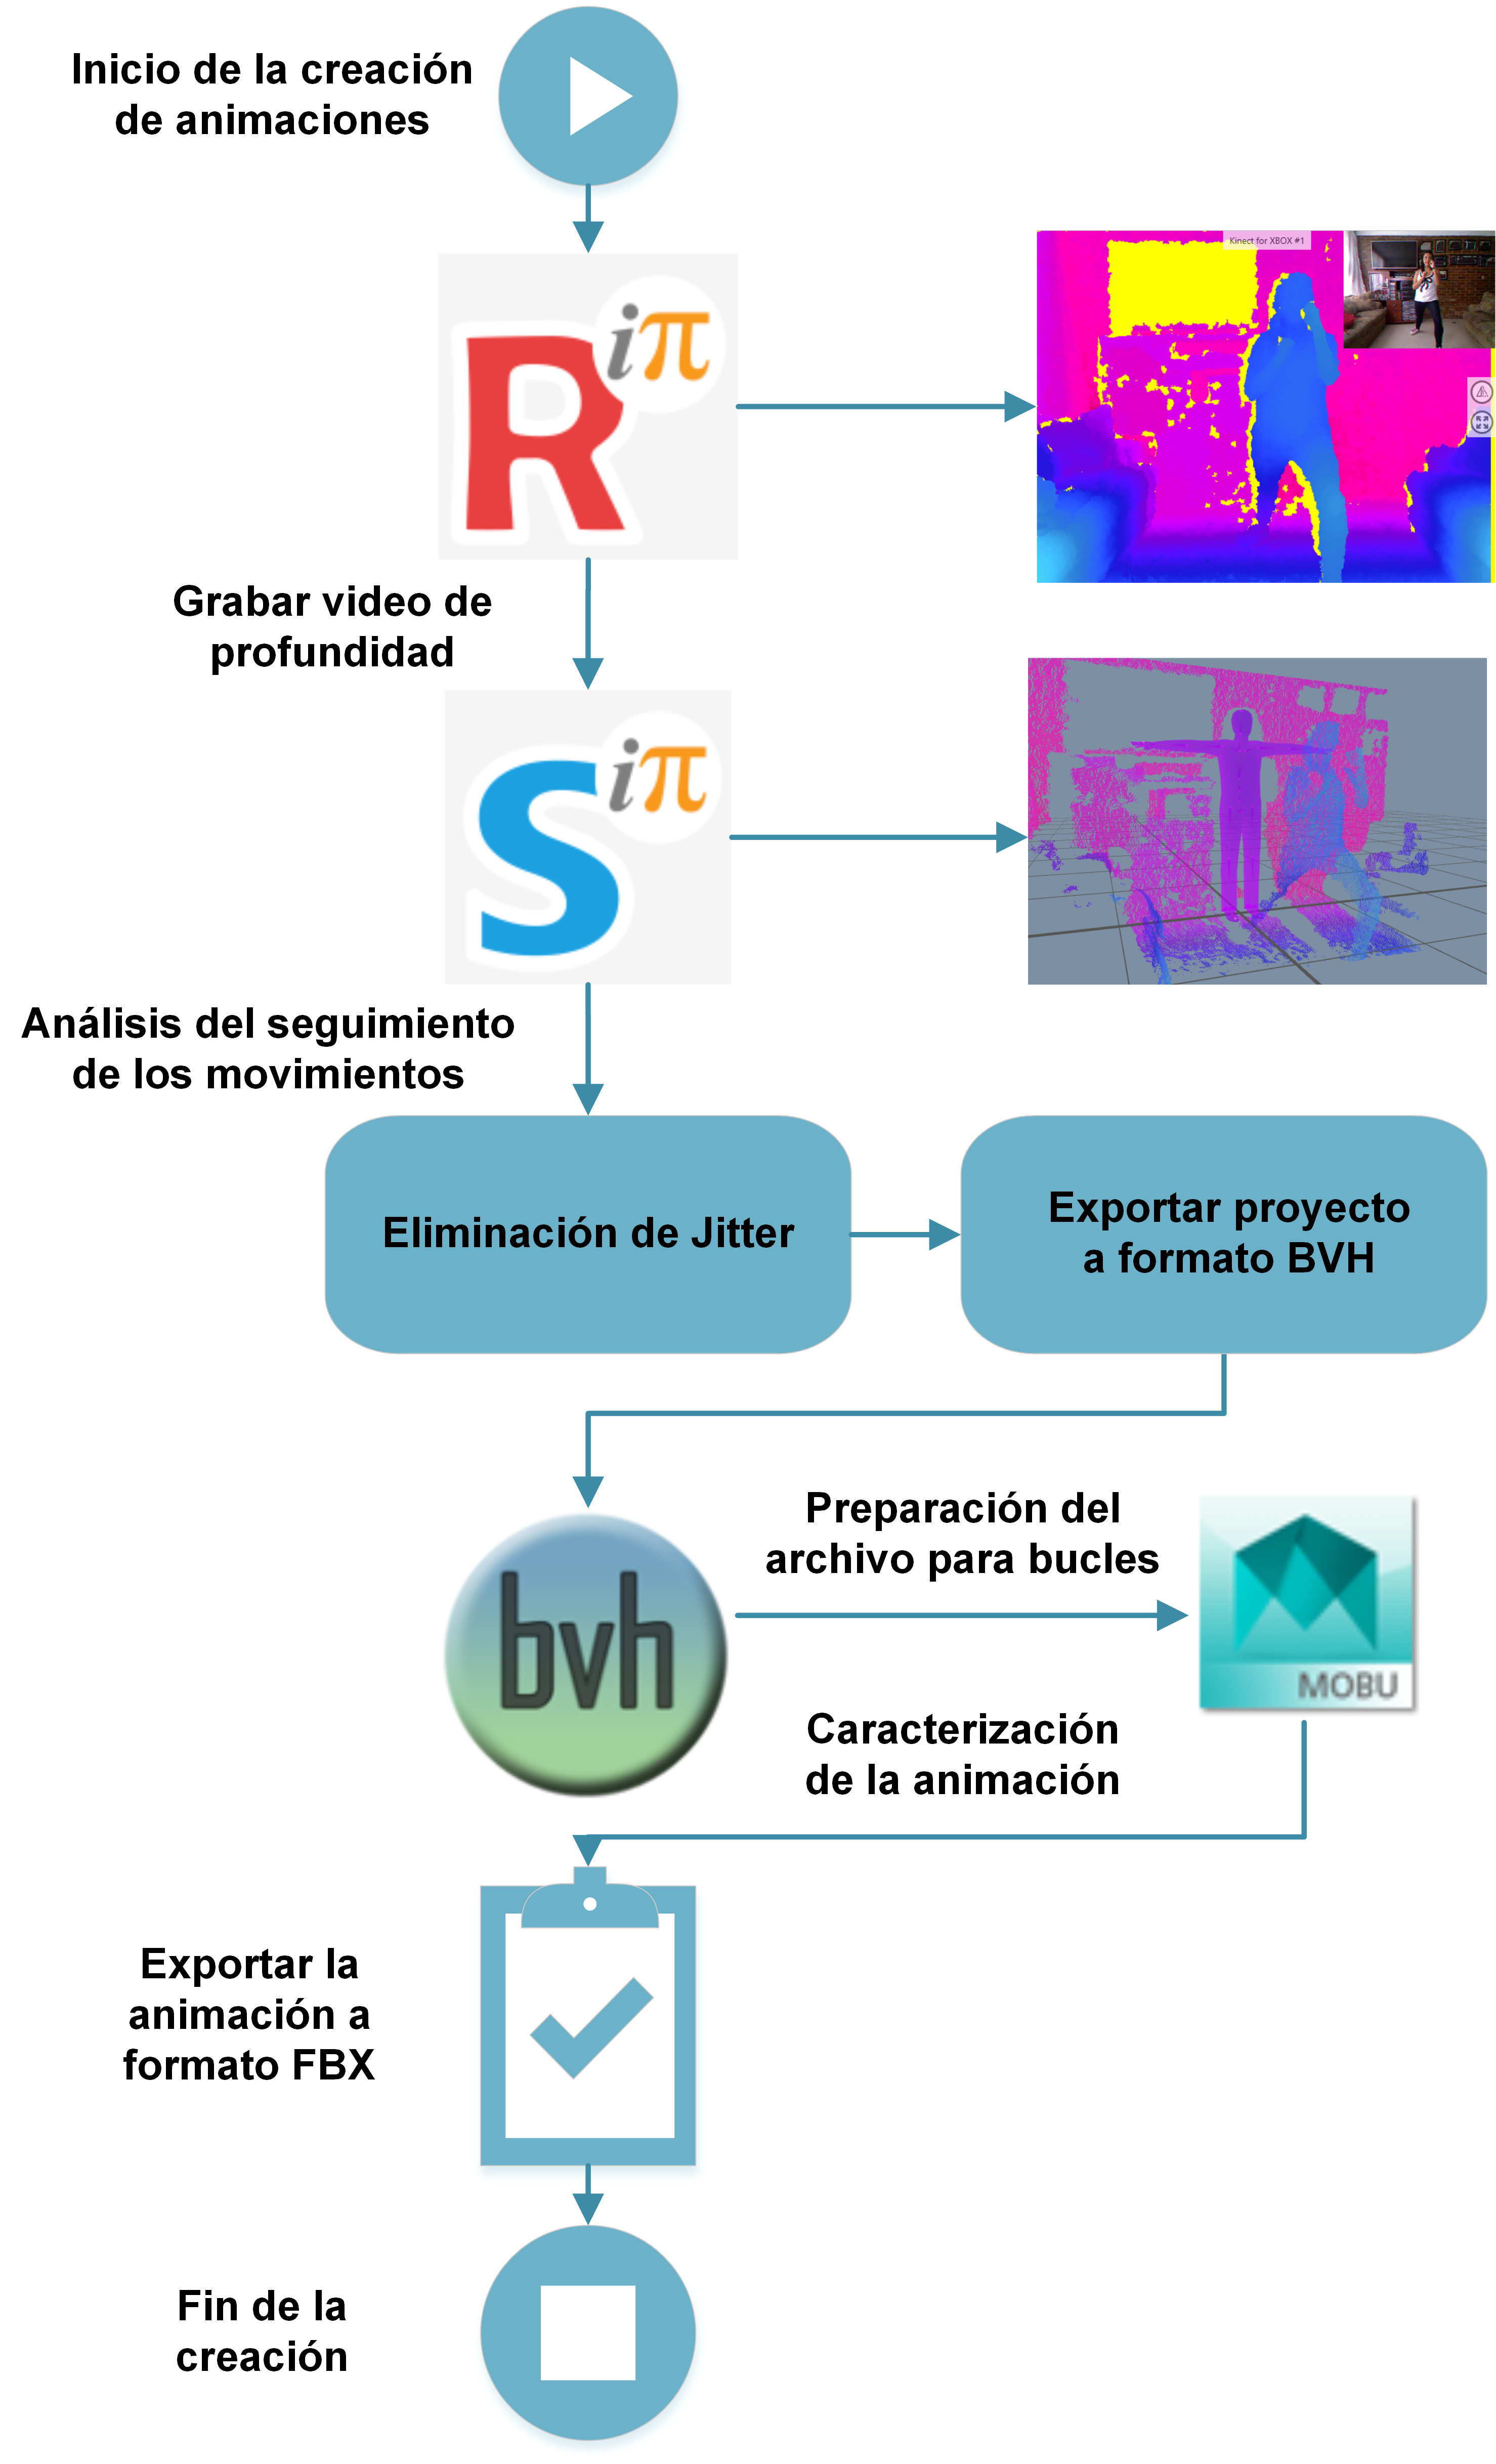
\includegraphics[scale=0.8]{./Figuras/Implementacion/Animaciones}
	\end{center}
	\caption{Proceso para generar una animación}
	\label{fig:Animaciones}
\end{figure}

% Describir el proceso si se requiere
\clearpage
\subsubsection{Implementación del algoritmo DTW}

El proceso realizado para la captura y validación de los movimientos se muestra a continuación, ver figura \ref{fig:ValidacionMovimiento} \nameref{fig:ValidacionMovimiento}.
\begin{figure}[H]%La h significa que la colocara cerca del texto
	\begin{center}
		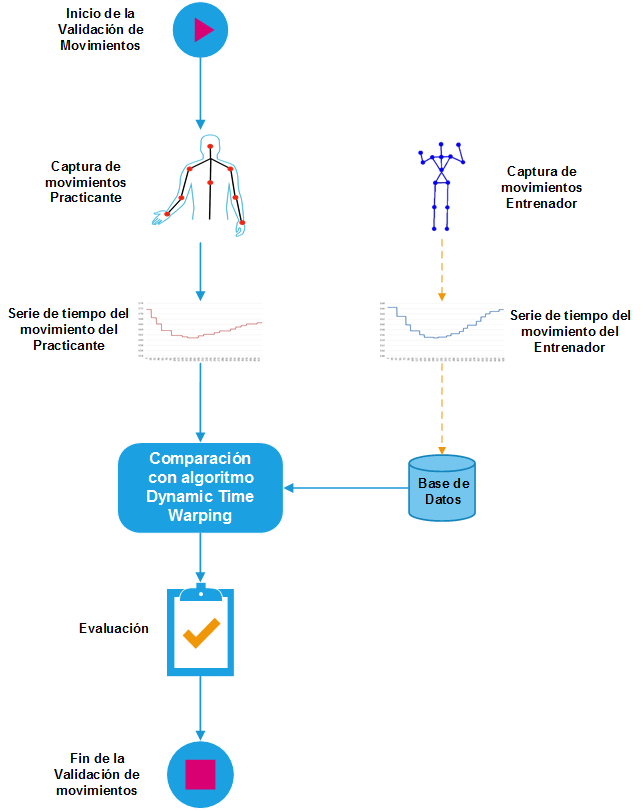
\includegraphics[scale=0.75]{./Figuras/Implementacion/ValidacionMovimiento}
	\end{center}
	\caption{Proceso de la captura y validación de movimientos}
	\label{fig:ValidacionMovimiento}
\end{figure}
\clearpage

A continuación se describe el proceso para la captura y validación de movimientos:\\

\textbf{Captura de movimientos del Practicante:}\\
Se utiliza el proceso de captura (ver sección \ref{sec:Captura} \nameref{sec:Captura}), para que el Practicante replique los ejercicios de calentamiento y los movimientos de técnica que se encuentren en la rutina seleccionada.\\

\textbf{Serie de tiempo de la captura de movimientos:}\\
Cuando se genera un movimiento por el usuario, los valores de cada una de las series de ángulos en tiempo por cada extremidad y por cada plano, se toman como los valores de una serie de tiempo, representándolo de la siguiente forma:\\
A= \{ a1, a2, a3, a4, a5,...an \}\\
B= \{ b1, b2, b3, b4, b5,...bm \}\\

Al tomar estos valores como una serie de tiempo, los puntos forman la siguiente representación gráfica, ver figura \ref{fig:Grafica1_Practicante} \nameref{fig:Grafica1_Practicante}. \\
\begin{figure}[H]%La h significa que la colocara cerca del texto
	\begin{center}
		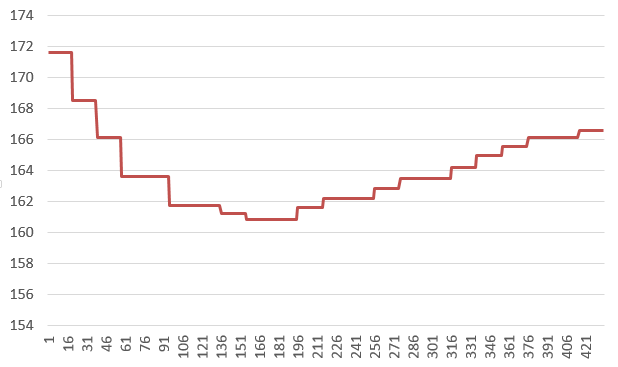
\includegraphics[scale=0.45]{./Figuras/Implementacion/Grafica1_Practicante}
	\end{center}
	\caption{Serie de Tiempo Practicante}
	\label{fig:Grafica1_Practicante}
\end{figure}

\textbf{Comparación con Algoritmo Dynamic Time Warping:}\\
La comparación se realiza utilizando el algoritmo de Dynamic Time Warping (ver sección \ref{sec:DTW} \nameref{sec:DTW}), a partir de la señal base, que es la serie de tiempo obtenida de la captura que realizó el Entrenador, la cual se encuentra almacenada en la base de datos.\\
Comparada con la serie de tiempo generada por el Practicante, como se observa en la figura \ref{fig:GraficaComparacionDTW} \nameref{fig:GraficaComparacionDTW}. \\

\begin{figure}[H]%La h significa que la colocara cerca del texto
	\begin{center}
		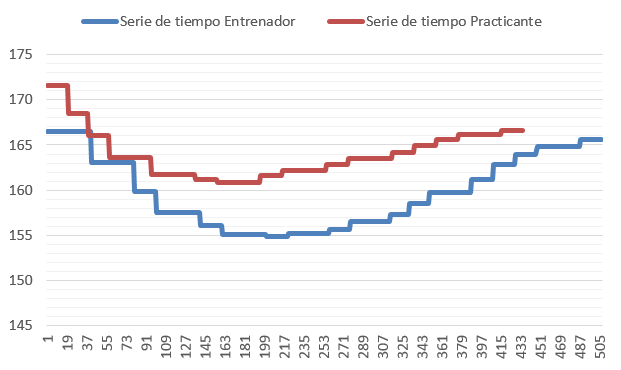
\includegraphics[scale=.45]{./Figuras/Implementacion/GraficaComparacionDTW}
	\end{center}
	\caption{Comparación de la series de tiempo de Entrenador y Practicante}
	\label{fig:GraficaComparacionDTW}
\end{figure}

\textbf{Evaluación:}\\
El valor resultante de la comparación se ocupa en la etapa de la evaluación, en donde de acuerdo al umbral definido para cada movimiento (ver sección \ref{sec:Umbral} \nameref{sec:Umbral}) genera el valor final de evaluación del movimiento.\\

\clearpage

\subsubsection{Pruebas}

\textbf{Registro de Practicantes:}\\
La siguiente pantalla muestra el correcto funcionamiento del registro de practicantes, se colocaron datos de muestra y un correo electrónico real creado para el registro de esta prueba.
\begin{figure}[H]%La h significa que la colocara cerca del texto
	\begin{center}
		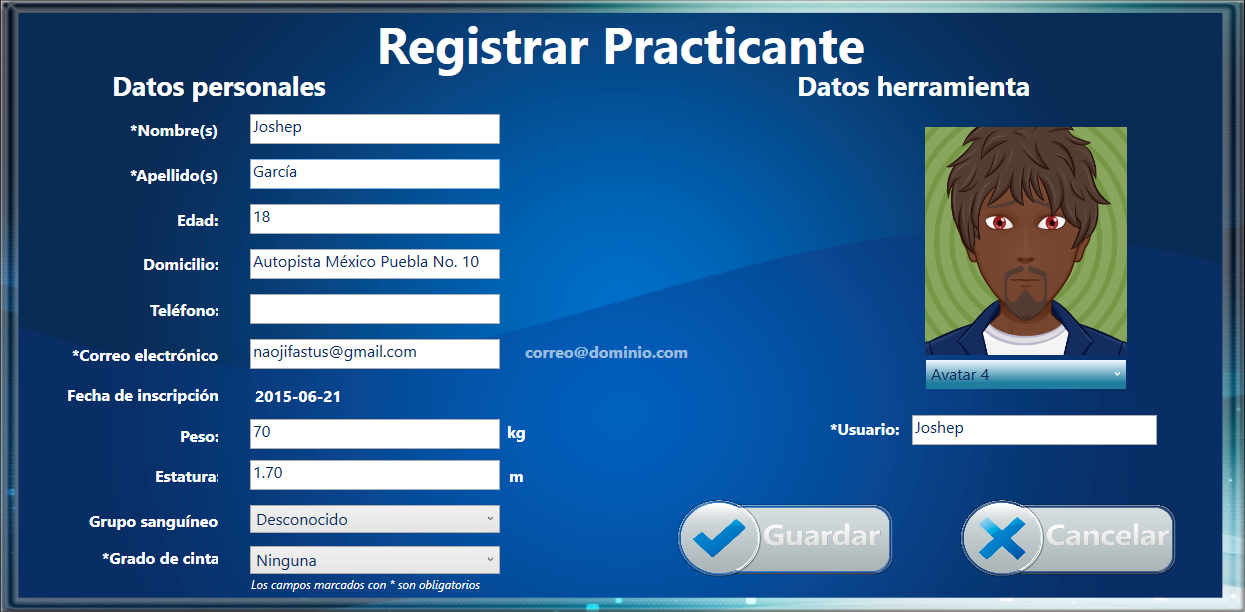
\includegraphics[scale=0.50]{./Figuras/Implementacion/Pruebas/Prueba_Registro_practicante}
	\end{center}
	\caption{Prueba de Registro de Practicante}
	\label{fig:Prueba_Registro_practicante}
\end{figure}

Una vez que los datos han sido capturados correctamente y el Practicante se ha dado de alta de manera exitosa, se muestra un mensaje de notificación y se envía un correo electrónico al nuevo Practicante con su nombre de usuario y su contraseña generada automáticamente por la herramienta.
\begin{figure}[H]
	\centering
	\subfloat[Mensaje de Registro exitoso]{
		\label{fig:Prueba_Registro_practicante-mensaje}
		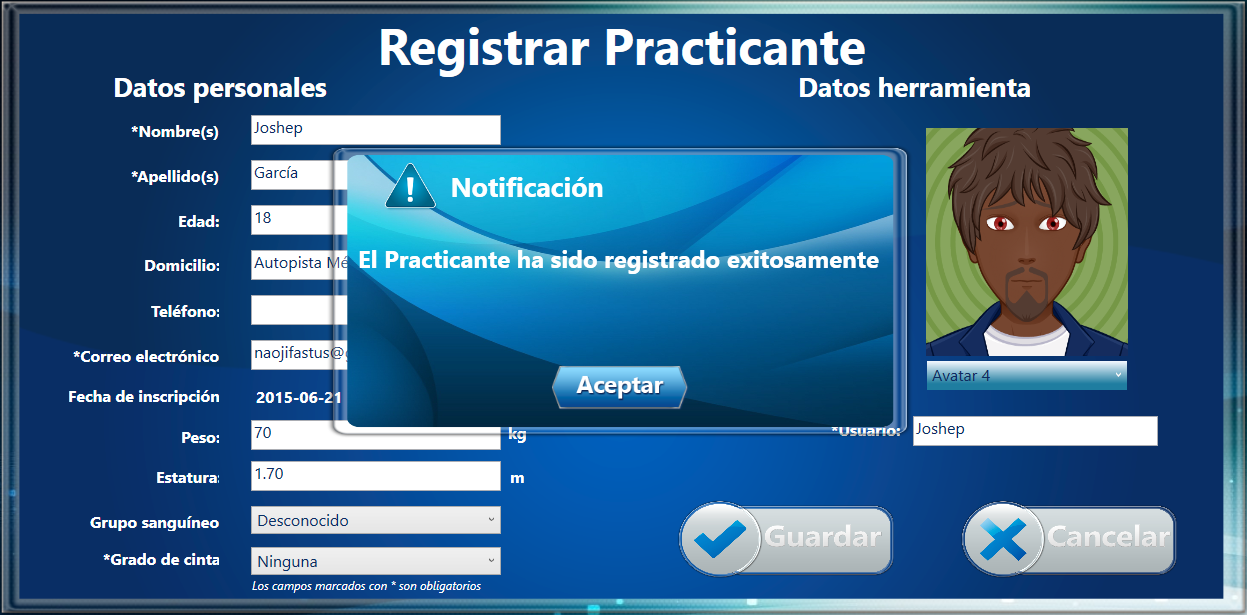
\includegraphics[width=8cm, height=7cm]{./Figuras/Implementacion/Pruebas/Prueba_Registro_practicante-mensaje}}
	\subfloat[Correo electrónico para el Practicante]{
		\label{fig:Prueba_Registro_practicante-correo}
		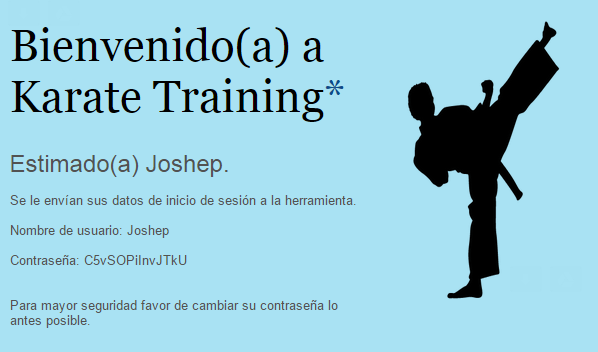
\includegraphics[width=8cm, height=7cm]{./Figuras/Implementacion/Pruebas/Prueba_Registro_practicante-correo}}
	\caption{Practicante registrado exitosamente}
	\label{fig:Prueba_Registro_practicante2}
\end{figure}
%------------------------------------------------------
\textbf{Registro de Rutinas:}\\
La siguiente pantalla muestra el correcto funcionamiento del registro de rutinas, que es realizado mediante la selección de los ejercicios y los movimientos registrados previamente, además del número de repeticiones para cada ejercicio y movimiento.
\begin{figure}[H]%La h significa que la colocara cerca del texto
	\begin{center}
		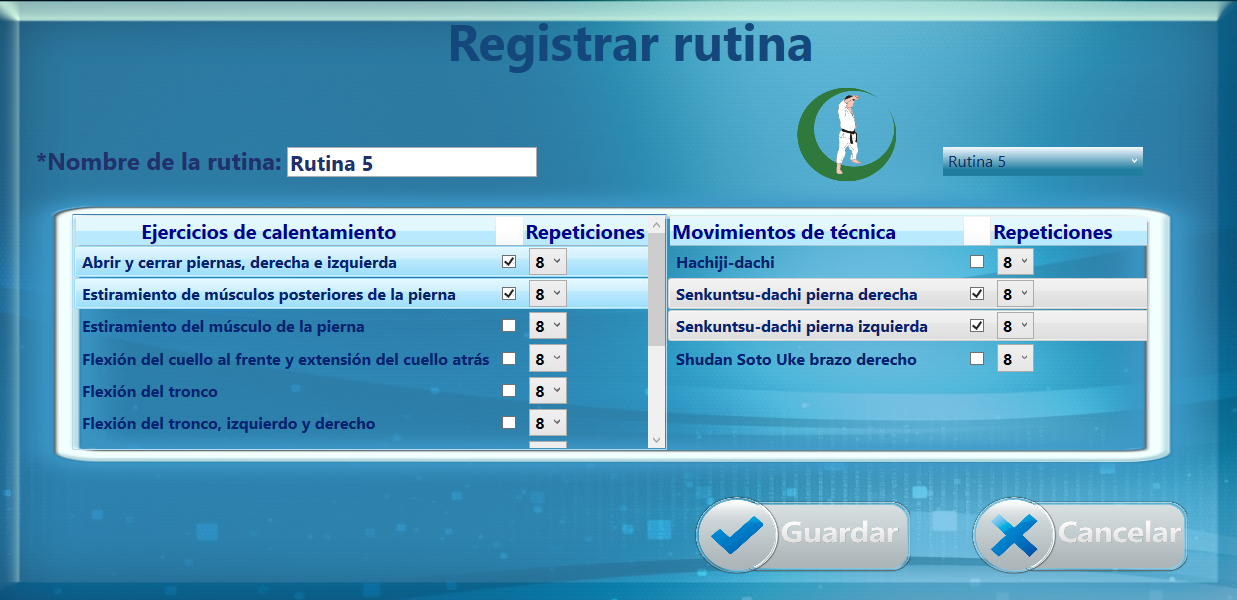
\includegraphics[scale=0.50]{./Figuras/Implementacion/Pruebas/Prueba_Registro_rutina}
	\end{center}
	\caption{Prueba de Registro de Rutinas}
	\label{fig:Prueba_Registro_rutina}
\end{figure}

Los datos de entrada cumplieron con el formato especificado en las reglas de negocio y la rutina se agregó exitosamente.
\begin{figure}[H]%La h significa que la colocara cerca del texto
	\begin{center}
		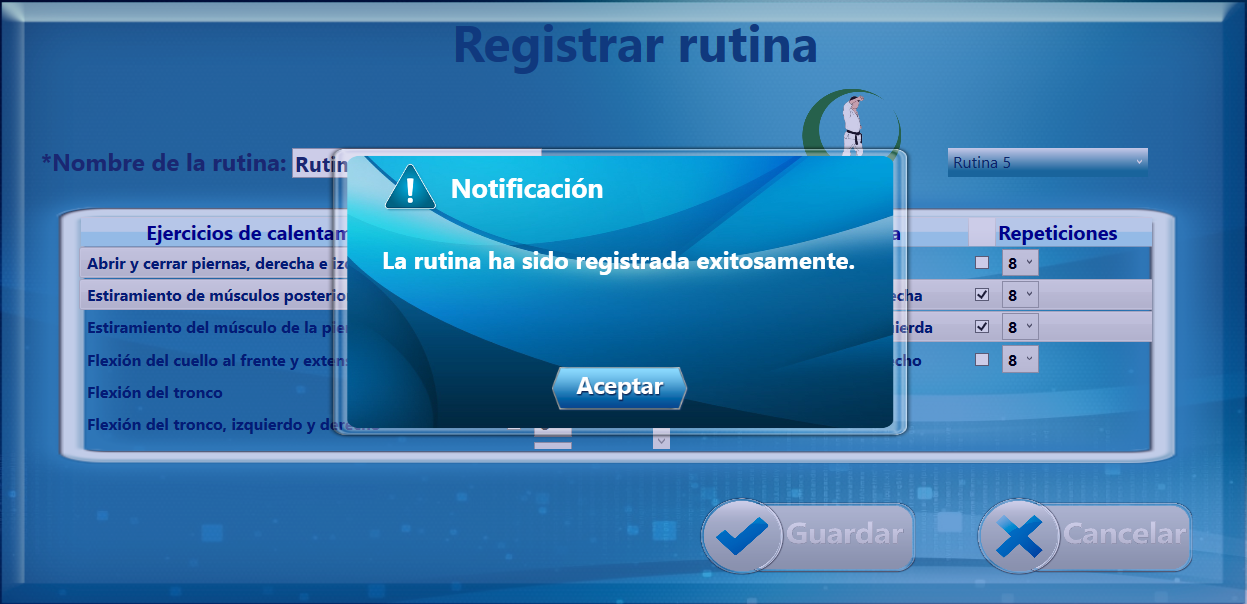
\includegraphics[scale=0.50]{./Figuras/Implementacion/Pruebas/Prueba_Registro_rutina-mensaje}
	\end{center}
	\caption{Practicante registrado exitosamente}
	\label{fig:Prueba_Registro_rutina-mensaje}
\end{figure}

%-------------------------------------------------------
\clearpage
\textbf{Captura y validación de movimientos Hachiji - dachi:}\\
A continuación se muestran los resultados de las pruebas que se hicieron a un grupo de 15 personas sin ningún conocimiento de Karate Do. Se les pidió replicar los movimientos que el Entrenador experto les marcaba, sin un entrenamiento previo.\\
\begin{figure}[H]%La h significa que la colocara cerca del texto
	\begin{center}
		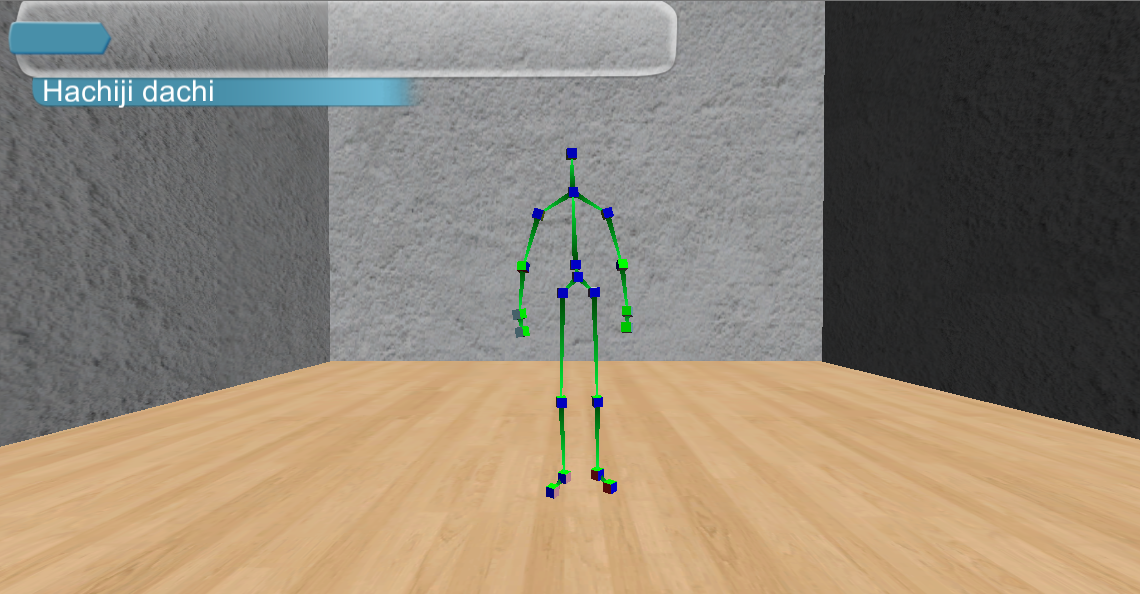
\includegraphics[scale=0.50]{./Figuras/Implementacion/Pruebas/Prueba_Capturar_movimientos}
	\end{center}
	\caption{Prueba de Capturar movimientos Hachiji - dachi}
	\label{fig:Prueba_Capturar_movimientos}
\end{figure}
En las tablas de Resultados Desviación Estándar-Entrenador, se puede observar el análisis de la desviación estándar y el promedio de 9 repeticiones del mismo movimiento del Entrenador, para poder obtener un indicador del umbral y con esto, la evaluación del movimiento de los Practicantes.
\begin{figure}[H]%La h significa que la colocara cerca del texto
	\begin{center}
		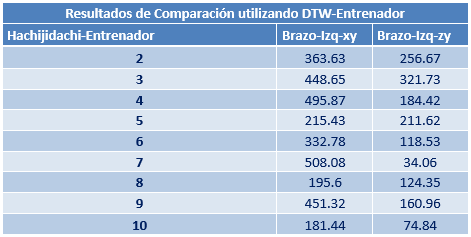
\includegraphics[scale=1]{./Figuras/Implementacion/Pruebas/Tablas/ResultadosDTW_Entrenador_Hachijidachi}
	\end{center}
	\caption{Resultados de la Comparación DTW Entrenador Hachiji - dachi}
	\label{fig:ResultadosDTW_Entrenador_Hachijidachi}
\end{figure}
\begin{figure}[H]%La h significa que la colocara cerca del texto
	\begin{center}
		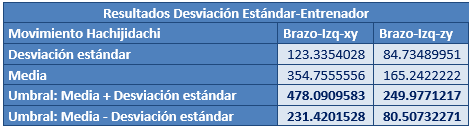
\includegraphics[scale=1]{./Figuras/Implementacion/Pruebas/Tablas/ResultadorDesvEstandar_Entrenador_Hachijidachi}
	\end{center}
	\caption{Resultados Desviación Estándar DTW Entrenador Hachiji - dachi}
	\label{fig:ResultadorDesvEstandar_Entrenador_Hachijidachi}
\end{figure}
En las tablas de Resultados de Comparación utilizando DTW- Practicantes, se pueden observar los resultados de la comparación de los movimientos de las personas inexpertas comparados con los movimientos del Entrenador experto.
\begin{figure}[H]%La h significa que la colocara cerca del texto
	\begin{center}
		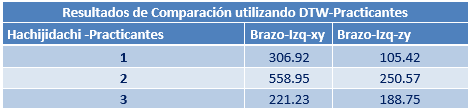
\includegraphics[scale=1]{./Figuras/Implementacion/Pruebas/Tablas/ResultadosDTW_Practicantes_Hachijidachi}
	\end{center}
	\caption{Resultados de la Comparación DTW Practicante Hachiji - dachi}
	\label{fig:ResultadosDTW_Practicantes_Hachijidachi}
\end{figure}
 Comparando el Valor del Umbral obtenido en la tabla de la desviación estándar del Entrenador, los cuales son:	478.090958 y 249.977122, respectivamente. Observamos que el Practicante 1 y el Practicante 3, se encuentran dentro del rango del umbral.
\begin{figure}[H]%La h significa que la colocara cerca del texto
	\begin{center}
		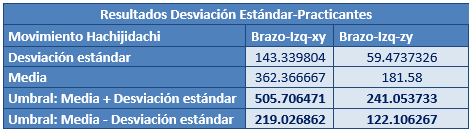
\includegraphics[scale=1]{./Figuras/Implementacion/Pruebas/Tablas/ResultadorDesvEstandar_Practicante_Hachijidachi}
	\end{center}
	\caption{Resultados Desviación Estándar DTW Practicante Hachiji - dachi}
	\label{fig:ResultadorDesvEstandar_Practicante_Hachijidachi}
\end{figure}

%-------------------------
\clearpage
\textbf{Captura y validación de movimientos Senkuntsu - dachi:}\\
\begin{figure}[H]%La h significa que la colocara cerca del texto
	\begin{center}
		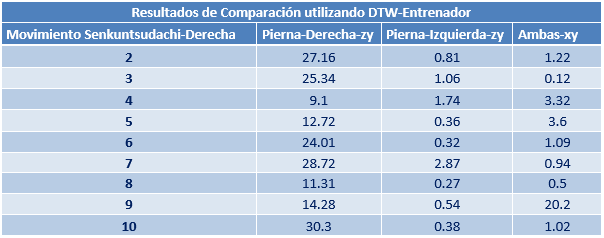
\includegraphics[scale=1]{./Figuras/Implementacion/Pruebas/Tablas/ResultadosDTW_Entrenador_Senkuntsudachi}
	\end{center}
	\caption{Resultados de la Comparación DTW Entrenador Senkuntsu - dachi}
	\label{fig:ResultadosDTW_Entrenador_Senkuntsudachi}
\end{figure}
\begin{figure}[H]%La h significa que la colocara cerca del texto
	\begin{center}
		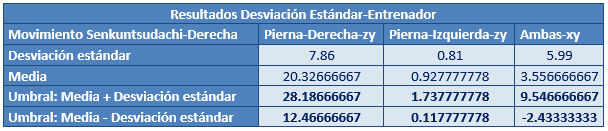
\includegraphics[scale=1]{./Figuras/Implementacion/Pruebas/Tablas/ResultadorDesvEstandar_Entrenador_Senkuntsudachi}
	\end{center}
	\caption{Resultados Desviación Estándar DTW Entrenador Senkuntsu - dachi}
	\label{fig:ResultadorDesvEstandar_Entrenador_Senkuntsudachi}
\end{figure}
\begin{figure}[H]%La h significa que la colocara cerca del texto
	\begin{center}
		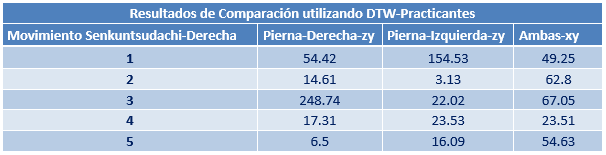
\includegraphics[scale=1]{./Figuras/Implementacion/Pruebas/Tablas/ResultadosDTW_Practicantes_Senkuntsudachi}
	\end{center}
	\caption{Resultados de la Comparación DTW Practicante Senkuntsu - dachi}
	\label{fig:ResultadosDTW_Practicantes_Senkuntsudachi}
\end{figure}
\begin{figure}[H]%La h significa que la colocara cerca del texto
	\begin{center}
		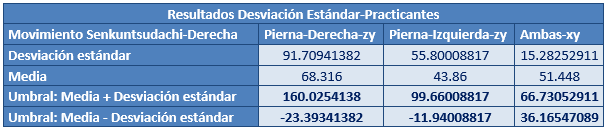
\includegraphics[scale=1]{./Figuras/Implementacion/Pruebas/Tablas/ResultadorDesvEstandar_Practicante_Senkuntsudachi}
	\end{center}
	\caption{Resultados Desviación Estándar DTW Practicante Senkuntsu - dachi}
	\label{fig:ResultadorDesvEstandar_Practicante_Senkuntsudachi}
\end{figure}
\textbf{Captura y validación de movimientos Senkuntsu - dachi Izquierda}\\
\begin{figure}[H]%La h significa que la colocara cerca del texto
	\begin{center}
		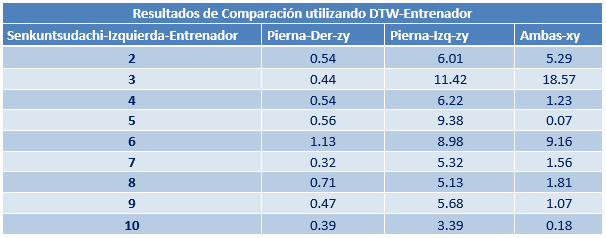
\includegraphics[scale=1]{./Figuras/Implementacion/Pruebas/Tablas/ResultadosDTW_Entrenador_Senkuntsudachi-Izquierdo}
	\end{center}
	\caption{Resultados de la Comparación DTW Entrenador Senkuntsu - dachi Izquierda}
	\label{fig:ResultadosDTW_Entrenador_Senkuntsudachi-Izquierdo}
\end{figure}
\begin{figure}[H]%La h significa que la colocara cerca del texto
	\begin{center}
		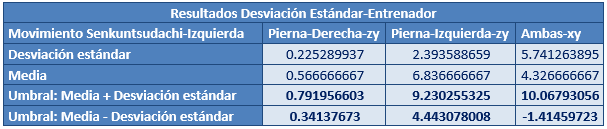
\includegraphics[scale=1]{./Figuras/Implementacion/Pruebas/Tablas/ResultadorDesvEstandar_Entrenador_Senkuntsudachi-Izquierdo}
	\end{center}
	\caption{Resultados Desviación Estándar DTW Entrenador Senkuntsu - dachi Izquierda}
	\label{fig:ResultadorDesvEstandar_Entrenador-Izquierdo}
\end{figure}
\begin{figure}[H]
	\centering
	\subfloat[Movimiendo Senkuntsu - dachi realizado por un Entrenador.]{
		\label{fig:CapturaProfesordeKarate}
		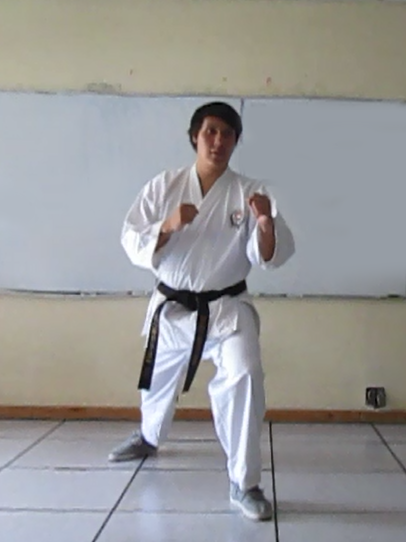
\includegraphics[width=7cm, height=8cm]{./Figuras/Implementacion/Pruebas/CapturaProfesordeKarate}}
	\subfloat[Movimiendo Senkuntsu - dachi realizado por una persona sin un entrenamiento previo.]{
		\label{fig:CapturaInexpertoenKarate}
		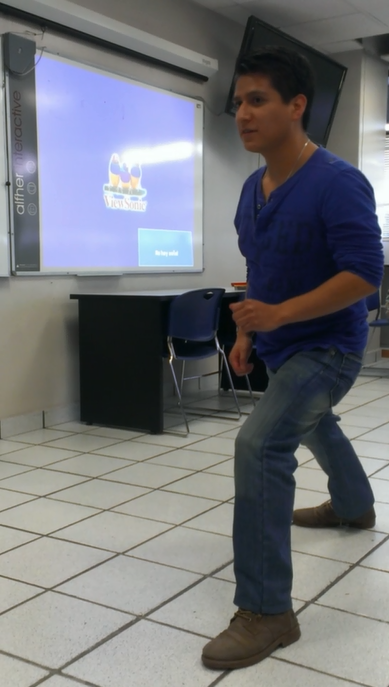
\includegraphics[width=5.5cm, height=8cm]{./Figuras/Implementacion/Pruebas/CapturaInexpertoenKarate}}
	\label{fig:CapturaPruebasKarate}
\end{figure}


%-------------------------
\clearpage
\textbf{Captura y validación de movimientos Shudan - soto - uke:}\\
\begin{figure}[H]%La h significa que la colocara cerca del texto
	\begin{center}
		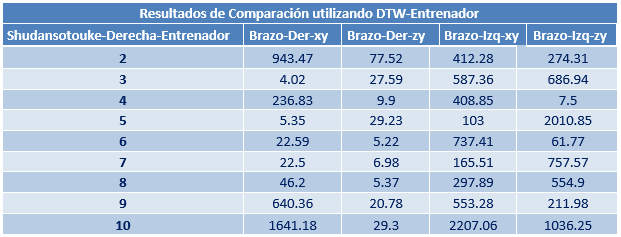
\includegraphics[scale=1]{./Figuras/Implementacion/Pruebas/Tablas/ResultadosDTW_Entrenador_Shudansotouke}
	\end{center}
	\caption{Resultados de la Comparación DTW Entrenador Shudan - soto - uke}
	\label{fig:ResultadosDTW_Entrenador_Shudansotouke}
\end{figure}
\begin{figure}[H]%La h significa que la colocara cerca del texto
	\begin{center}
		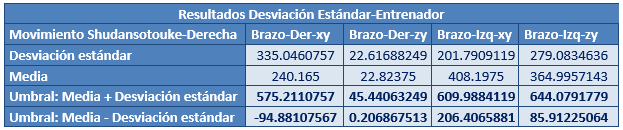
\includegraphics[scale=1]{./Figuras/Implementacion/Pruebas/Tablas/ResultadorDesvEstandar_Entrenador_Shudansotouke}
	\end{center}
	\caption{Resultados Desviación Estándar DTW Entrenador Shudan - soto - uke}
	\label{fig:ResultadorDesvEstandar_Entrenador_Shudansotouke}
\end{figure}
Los resultados arrojan que la mayoría de las personas realizaron mal el movimiento de técnica marcado por el Entrenador.
\begin{figure}[H]%La h significa que la colocara cerca del texto
	\begin{center}
		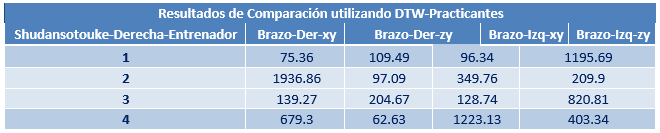
\includegraphics[scale=1]{./Figuras/Implementacion/Pruebas/Tablas/ResultadosDTW_Practicantes_Shudansotouke}
	\end{center}
	\caption{Resultados de la Comparación DTW Practicante Shudan - soto - uke}
	\label{fig:ResultadosDTW_Practicantes_Shudansotouke}
\end{figure}
\begin{figure}[H]%La h significa que la colocara cerca del texto
	\begin{center}
		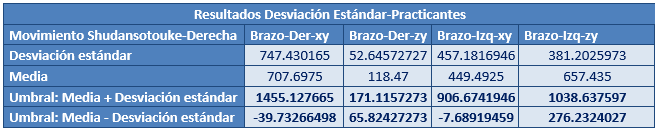
\includegraphics[scale=1]{./Figuras/Implementacion/Pruebas/Tablas/ResultadorDesvEstandar_Practicante_Shudansotouke}
	\end{center}
	\caption{Resultados Desviación Estándar DTW Practicante Shudan - soto - uke}
	\label{fig:ResultadorDesvEstandar_Practicante_Shudansotouke}
\end{figure}
\textbf{Captura y validación de movimientos Shudan - soto - uke Izquierda:}\\
\begin{figure}[H]%La h significa que la colocara cerca del texto
	\begin{center}
		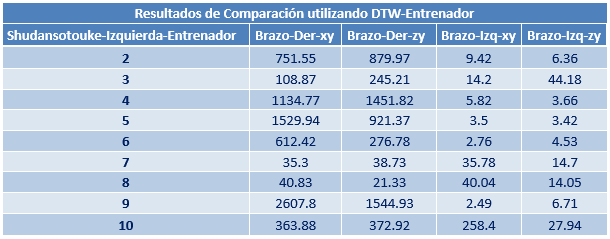
\includegraphics[scale=1]{./Figuras/Implementacion/Pruebas/Tablas/ResultadosDTW_Entrenador_Shudansotouke-Izquierdo}
	\end{center}
	\caption{Resultados de la Comparación DTW Entrenador Shudan - soto - uke Izquierda}
	\label{fig:ResultadosDTW_Entrenador_Shudansotouke-Izquierdo}
\end{figure}
\begin{figure}[H]%La h significa que la colocara cerca del texto
	\begin{center}
		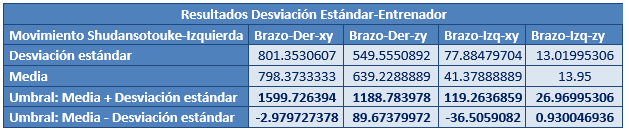
\includegraphics[scale=1]{./Figuras/Implementacion/Pruebas/Tablas/ResultadorDesvEstandar_Entrenador_Shudansotouke-Izquierdo}
	\end{center}
	\caption{Resultados Desviación Estándar DTW Entrenador Shudan - soto - uke Izquierda}
	\label{fig:ResultadorDesvEstandar_Entrenador_Shudansotouke-Izquierdo}
\end{figure}

%-------------------------
\clearpage
\textbf{Captura y validación de movimientos Gedan - barai - uke:}\\
\begin{figure}[H]%La h significa que la colocara cerca del texto
	\begin{center}
		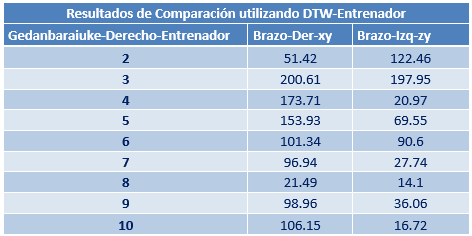
\includegraphics[scale=1]{./Figuras/Implementacion/Pruebas/Tablas/ResultadosDTW_Entrenador_Gedanbaraiuke}
	\end{center}
	\caption{Resultados de la Comparación DTW Entrenador Gedan - barai - uke}
	\label{fig:ResultadosDTW_Entrenador_Gedanbaraiuke}
\end{figure}
\begin{figure}[H]%La h significa que la colocara cerca del texto
	\begin{center}
		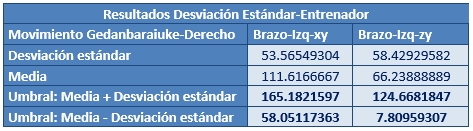
\includegraphics[scale=1]{./Figuras/Implementacion/Pruebas/Tablas/ResultadorDesvEstandar_Entrenador_Gedanbaraiuke}
	\end{center}
	\caption{Resultados Desviación Estándar DTW Entrenador Gedan - barai - uke}
	\label{fig:ResultadorDesvEstandar_Entrenador_Gedanbaraiuke}
\end{figure}
\begin{figure}[H]%La h significa que la colocara cerca del texto
	\begin{center}
		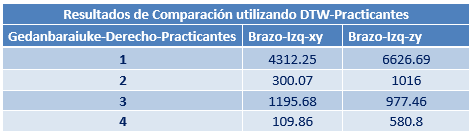
\includegraphics[scale=1]{./Figuras/Implementacion/Pruebas/Tablas/ResultadosDTW_Practicante_Gedanbaraiuke}
	\end{center}
	\caption{Resultados de la Comparación DTW Practicante Gedan - barai - uke}
	\label{fig:ResultadosDTW_Practicante_Gedanbaraiuke}
\end{figure}
\begin{figure}[H]%La h significa que la colocara cerca del texto
	\begin{center}
		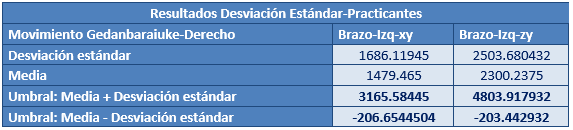
\includegraphics[scale=1]{./Figuras/Implementacion/Pruebas/Tablas/ResultadorDesvEstandar_Practicante_Gedanbaraiuke}
	\end{center}
	\caption{Resultados Desviación Estándar DTW Practicante Gedan - barai - uke}
	\label{fig:ResultadorDesvEstandar_Practicante_Gedanbaraiuke}
\end{figure}
\textbf{Captura y validación de movimientos Gedan - barai - uke Izquierda:}\\
\begin{figure}[H]%La h significa que la colocara cerca del texto
	\begin{center}
		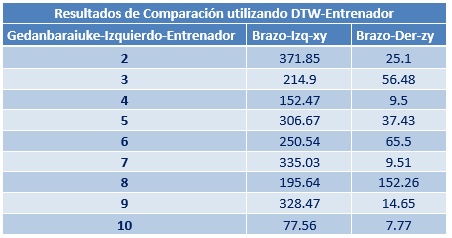
\includegraphics[scale=1]{./Figuras/Implementacion/Pruebas/Tablas/ResultadosDTW_Entrenador_Gedanbaraiuke-Izquierdo}
	\end{center}
	\caption{Resultados de la Comparación DTW Entrenador Gedan - barai - uke Izquierda}
	\label{fig:ResultadosDTW_Entrenador_Gedanbaraiuke-Izquierdo}
\end{figure}
\begin{figure}[H]%La h significa que la colocara cerca del texto
	\begin{center}
		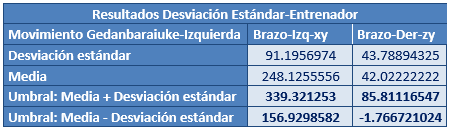
\includegraphics[scale=1]{./Figuras/Implementacion/Pruebas/Tablas/ResultadorDesvEstandar_Entrenador_Gedanbaraiuke-Izquierdo}
	\end{center}
	\caption{Resultados Desviación Estándar DTW Entrenador Gedan - barai - uke Izquierda}
	\label{fig:ResultadorDesvEstandar_Entrenador_Gedanbaraiuke-Izquierdo}
\end{figure}
\clearpage

%-------------------------
\textbf{Captura y validación de movimientos Mae - geri:}\\
\begin{figure}[H]%La h significa que la colocara cerca del texto
	\begin{center}
		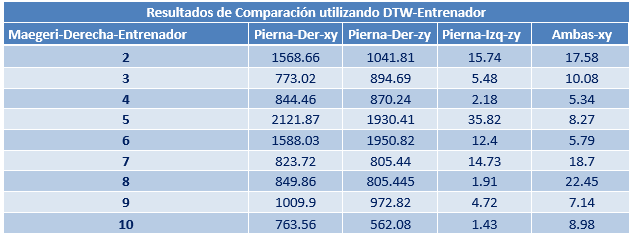
\includegraphics[scale=1]{./Figuras/Implementacion/Pruebas/Tablas/ResultadosDTW_Entrenador_Maegeri}
	\end{center}
	\caption{Resultados de la Comparación DTW Entrenador Mae - geri}
	\label{fig:ResultadosDTW_Entrenador_Maegeri}
\end{figure}
\begin{figure}[H]%La h significa que la colocara cerca del texto
	\begin{center}
		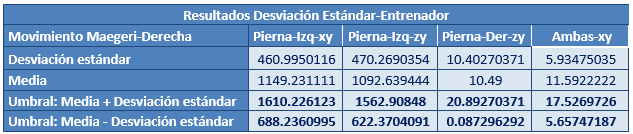
\includegraphics[scale=1]{./Figuras/Implementacion/Pruebas/Tablas/ResultadorDesvEstandar_Entrenador_Maegeri}
	\end{center}
	\caption{Resultados Desviación Estándar DTW Entrenador Mae - geri}
	\label{fig:ResultadosDTW_Entrenador_Maegeri}
\end{figure}
\textbf{Captura y validación de movimientos Mae - geri Izquierda:}\\
\begin{figure}[H]%La h significa que la colocara cerca del texto
	\begin{center}
		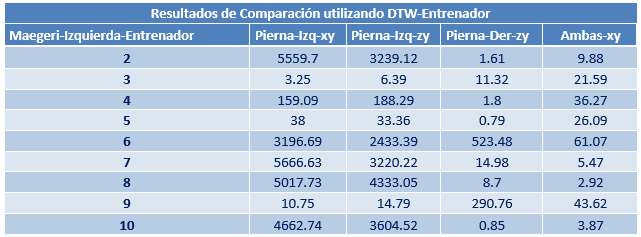
\includegraphics[scale=1]{./Figuras/Implementacion/Pruebas/Tablas/ResultadosDTW_Entrenador_Maegeri-Izquierdo}
	\end{center}
	\caption{Resultados de la Comparación DTW Entrenador Mae - geri Izquierda}
	\label{fig:ResultadosDTW_Entrenador_Maegeri-Izquierdo}
\end{figure}
\begin{figure}[H]%La h significa que la colocara cerca del texto
	\begin{center}
		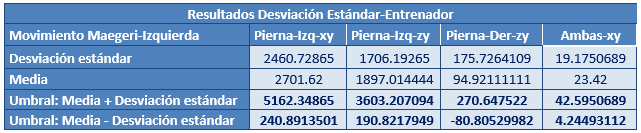
\includegraphics[scale=1]{./Figuras/Implementacion/Pruebas/Tablas/ResultadorDesvEstandar_Entrenador_Maegeri-Izquierdo}
	\end{center}
	\caption{Resultados Desviación Estándar DTW Entrenador Mae - geri Izquierda}
	\label{fig:ResultadosDTW_Entrenador_Maegeri-Izquierdo}
\end{figure}
\clearpage

%-------------------------
\textbf{Captura y validación de movimientos Seiken - tsuki:}\\
\begin{figure}[H]%La h significa que la colocara cerca del texto
	\begin{center}
		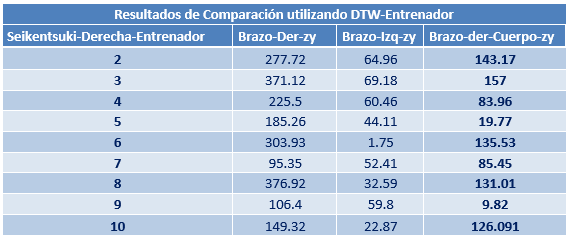
\includegraphics[scale=1]{./Figuras/Implementacion/Pruebas/Tablas/ResultadosDTW_Entrenador_Seikentsuki}
	\end{center}
	\caption{Resultados de la Comparación DTW Entrenador Seiken - tsuki}
	\label{fig:ResultadosDTW_Entrenador_Seikentsuki}
\end{figure}
\begin{figure}[H]%La h significa que la colocara cerca del texto
	\begin{center}
		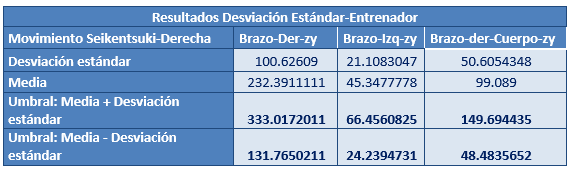
\includegraphics[scale=1]{./Figuras/Implementacion/Pruebas/Tablas/ResultadorDesvEstandar_Entrenador_Seikentsuki}
	\end{center}
	\caption{Resultados Desviación Estándar DTW Entrenador Seiken - tsuki}
	\label{fig:ResultadosDTW_Entrenador_Seikentsuki}
\end{figure}
\textbf{Captura y validación de movimientos Seiken - tsuki Izquierda:}\\
\begin{figure}[H]%La h significa que la colocara cerca del texto
	\begin{center}
		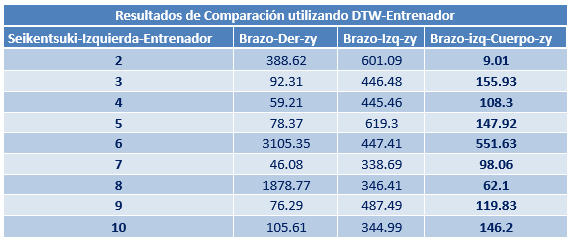
\includegraphics[scale=1]{./Figuras/Implementacion/Pruebas/Tablas/ResultadosDTW_Entrenador_Seikentsuki-Izquierdo}
	\end{center}
	\caption{Resultados de la Comparación DTW Entrenador Seiken - tsuki Izquierda}
	\label{fig:ResultadosDTW_Entrenador_Seikentsuki-Izquierdo}
\end{figure}
\begin{figure}[H]%La h significa que la colocara cerca del texto
	\begin{center}
		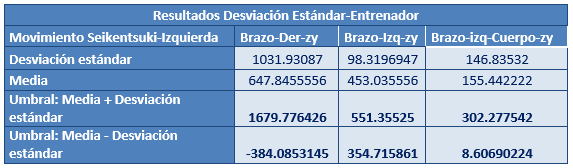
\includegraphics[scale=1]{./Figuras/Implementacion/Pruebas/Tablas/ResultadorDesvEstandar_Entrenador_Seikentsuki-Izquierdo}
	\end{center}
	\caption{Resultados Desviación Estándar DTW Entrenador Seiken - tsuki Izquierda}
	\label{fig:ResultadosDTW_Entrenador_Seikentsuki-Izquierdo}
\end{figure}
\clearpage

%-------------------------
\textbf{Captura y validación de movimientos Yodan - age - uke:}\\
\begin{figure}[H]%La h significa que la colocara cerca del texto
	\begin{center}
		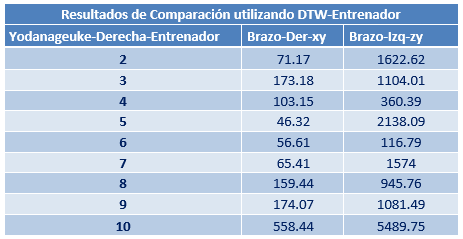
\includegraphics[scale=1]{./Figuras/Implementacion/Pruebas/Tablas/ResultadosDTW_Entrenador_Yodanageuke}
	\end{center}
	\caption{Resultados de la Comparación DTW Entrenador Yodan - age - uke}
	\label{fig:ResultadosDTW_Entrenador_Yodanageuke}
\end{figure}
\begin{figure}[H]%La h significa que la colocara cerca del texto
	\begin{center}
		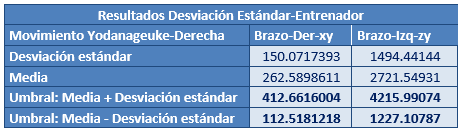
\includegraphics[scale=1]{./Figuras/Implementacion/Pruebas/Tablas/ResultadorDesvEstandar_Entrenador_Yodanageuke}
	\end{center}
	\caption{Resultados Desviación Estándar DTW Entrenador Yodan - age - uke}
	\label{fig:ResultadosDTW_Entrenador_Yodanageuke}
\end{figure}
\textbf{Captura y validación de movimientos Yodan - age - uke Izquierda:}\\
\begin{figure}[H]%La h significa que la colocara cerca del texto
	\begin{center}
		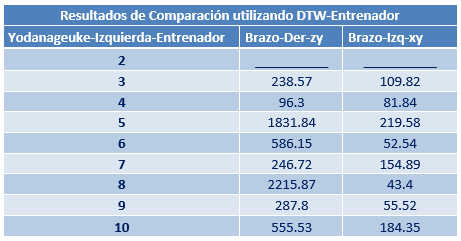
\includegraphics[scale=1]{./Figuras/Implementacion/Pruebas/Tablas/ResultadosDTW_Entrenador_Yodanageuke-Izquierdo}
	\end{center}
	\caption{Resultados de la Comparación DTW Entrenador Yodan - age - uke Izquierda}
	\label{fig:ResultadosDTW_Entrenador_Yodanageuke-Izquierdo}
\end{figure}
\begin{figure}[H]%La h significa que la colocara cerca del texto
	\begin{center}
		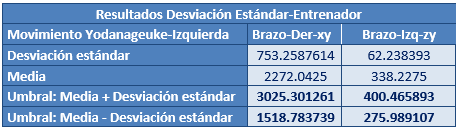
\includegraphics[scale=1]{./Figuras/Implementacion/Pruebas/Tablas/ResultadorDesvEstandar_Entrenador_Yodanageuke-Izquierdo}
	\end{center}
	\caption{Resultados Desviación Estándar DTW Entrenador Yodan - age - uke Izquierda}
	\label{fig:ResultadosDTW_Entrenador_Yodanageuke-Izquierdo}
\end{figure}

%-------------------------

En la mayoría de los resultados arrojados en las tablas comparativas, los valores de la comparación utilizando el algoritmo DTW, respecto los almacenados previamente por el Entrenador, rebasan el umbral que se definió para cada movimiento de acuerdo a las desviaciones estándar y el promedio de los movimientos del Entrenador (ver sección \ref{sec:Umbral} \nameref{sec:Umbral}).\\
